% -*- LaTeX -*-
% -*- coding: utf-8 -*-
%
% ~~~~~~~~~~~~~~~~~~~~~~~~~~~~~~~~~~~~~~~~~~~~~~~~~~~~~~~~~~~~~~~~~~~~~~~~~~~~~~
%
%                             michael a.g. aïvázis
%                      california institute of technology
%                      (c) 1998-2010  all rights reserved
%
% ~~~~~~~~~~~~~~~~~~~~~~~~~~~~~~~~~~~~~~~~~~~~~~~~~~~~~~~~~~~~~~~~~~~~~~~~~~~~~~
%

\lecture{Overview of algorithms}{20100106}

% --------------------------------------
% informal definitions of algorithm
\begin{frame}[fragile]
%
  \frametitle{Algorithms}
%
  \begin{itemize}
%
  \item Informally, an algorithm can be viewed as
    \begin{itemize}
    \item a well-defined computational procedure that
      \begin{itemize}
      \item takes a set of values as input
      \item produces a set of values as output
      \end{itemize}
    \item a solution to a computational problem
      \begin{itemize}
      \item whose statement specifies the intended relationship between inputs and outputs
      \item and the algorithm being the specific computational procedure that achieves this
        relationship
      \end{itemize}
    \end{itemize}
%
  \item the prototypical computational problem is {\em sorting}
    \begin{itemize}
    \item problem specification
      \begin{itemize}
      \item input: a sequence $S$ of $n$ numbers $(s_{0}, s_{1}, \ldots, s_{n})$
      \item output: a permutation $S'$ of the input sequence $(s'_{0}, s'_{1}, \ldots, s'_{n})$
      \item constraint: the elements of the output sequence must satisfy 
        \[ s'_{0} \leq s_{1}' \leq \ldots \leq s_{n}'\]
      \end{itemize}
    \item problem instance: $S = (0, \pi, 1, e, 2, 16)$
    \item invalid input: $(0, i, 1)$
      \begin{itemize}
      \item why is this bad? which implicit property of $S$ does it violate?  what is the set
        of valid inputs?
      \end{itemize}
    \end{itemize}
%
  \end{itemize}
%
\end{frame}

% --------------------------------------
% algorithm correctness
\begin{frame}[fragile]
%
  \frametitle{Correctness}
%
  \begin{itemize}
%
  \item once again informally, an algorithm is {\em correct} if
    \begin{itemize}
    \item it terminates for all valid input
    \item upon termination on valid input, the output satisfies the constraints expressed in
      the problem statement
    \end{itemize}
%
  \item equivalently, we say that the algorithm {\em solves} the computational problem
%
  \item after correctness has been established, algorithms are classified according to their
    demands on computational resources
    \begin{itemize}
    \item running time complexity
      \begin{itemize}
      \item a measure of the number of instructions necessary to solve the problem
      \end{itemize}
    \item and, occasionally
      \begin{itemize}
      \item amount of auxiliary storage
      \item network bandwidth or other communication infrastructure requirements
      \item for parallel algorithms: speedup and efficiency
      \end{itemize}
    \end{itemize}
%
  \item algorithms are often specified using {\em pseudoce}
    \begin{itemize}
      \item a loose language with mostly notational constraints
      \item a mixture of reasonable looking code with whatever expressive method  makes the
        point clear
      \item hence, the use of human languages to convey meaning that might be too difficult to
        code up, or would obscure the point, is perfectly acceptable
    \end{itemize}
%
  \end{itemize}
%
\end{frame}



% --------------------------------------
% the INSERTION-SORT algorithm
\begin{frame}[fragile]
%
  \frametitle{A sorting algorithm}
%
    \begin{center}
      \begin{minipage}{.75\linewidth}
        \begin{algorithm}[H]
          \label{alg:insertion-sort}
%
          \dontprintsemicolon
          %\nocaptionofalgo
          \setalcaphskip{0ex}
%
          \caption{\insertionsort($S$)}
          \vspace{.5em}
%
          \For{$j \leftarrow 2$  \KwTo length[S]}{
            $key \leftarrow S[j]$ \;
            $i \leftarrow j-1$ \;
            \While{$i > 0$ \KwAnd $S[i] > key$}{
              $S[i+1] \leftarrow S[i]$ \;
              $i \leftarrow i-1$ \;
            }
            $S[i+1] \leftarrow key$
          }
%
          \vspace{.5em}
%
        \end{algorithm}
      \end{minipage}
    \end{center}
%
  \begin{itemize}
%
  \item valid inputs:
    \begin{itemize}
    \item empty sequence, singlet, other sequences of finite length
    \item what kinds of objects in $S$?
    \end{itemize}
%
  \item walk through it by hand with $S = (5, 2, 4, 6, 1, 3)$
%
  \end{itemize}
%
\end{frame}

% --------------------------------------
% pseudocode
\begin{frame}[fragile]
%
  \frametitle{Pseudocode conventions}
%
  \begin{itemize}
  \item the symbol ``$\triangleright$'' indicates a comment through to the end of the line
  \item block structure is indicated by the indentation level
  \item all variables are local; no global variables, unless explicitly marked
  \item $i \leftarrow j \leftarrow k$ assigns the rightmost expression to all the other
    variables
  \item indexing: $S[i]$; slicing: $S[i .. j]$
  \item conditionals, looping constructs, function calls should be familiar
  \item compound objects have attributes or fields that are referenced using indexing,
    e.g. $length[S]$
  \item variables assigned to objects or containers are references
  \item parameters passed to procedures {\em by assignment}
  \end{itemize}
%
\end{frame}
        
% --------------------------------------
% python implementation of insertion-sort
\begin{frame}[fragile]
%
  \frametitle{Python implementation}
%
  \begin{itemize}
%
  \item direct translation of pseudocode in python, with no attempt to improve
%
  \begin{center}
    \begin{minipage}[h]{.75\linewidth}
      \begin{python}[%
        label={lst:insertion-sort:python},
        caption={Python implementation of insertion\_sort}
]
%
def insertion_sort(S):
    for j in range(1, len(S)):
        key = S[j]
        i = j-1
        while i>=0 and S[i]>key:
            S[i+1] = S[i]
            i = i-1
        S[i+1] = key
      \end{python}
    \end{minipage}
  \end{center}
%
  \item minor adjustments to loop indices are required since python lists are zero based
  \end{itemize}
%
\end{frame}

% --------------------------------------
% algorithm analysis
\begin{frame}[fragile]
%
  \frametitle{Analyzing algorithms}
%
  \begin{itemize}
%
  \item algorithm analysis is the computation of resource requirements
    \begin{itemize}
      \item memory, communication bandwidth, {\em computational time}
    \end{itemize}
%
  \item need a model for the implementation environment
    \begin{itemize}
      \item RAM: {\em random access machine}
      \item an abstraction of a single processor sequential execution machine that has access
        to a single block of memory with uniform access cost
      \item even though the model is extermely simple, algorithm analysis remains a hard
        problem, full of subtleties
    \end{itemize}
%
    \item in general, we seek to relate the running time to input size
      \begin{itemize}
        \item definition of input size is problem dependent -- could be number of items to sort,
          or number of grid points in a mesh, etc.
        \item running time is proportional to the number of primitive steps executed
        \item different lines have different costs
        \item but each execution of a given line is assumed to cost the same
      \end{itemize}
%
    \item {\em exercise}: decorate \algref{insertion-sort} with the number of times each line is
      executed
%
  \end{itemize}
%
\end{frame}

% --------------------------------------
% complexity of insertion-sort
\begin{frame}[fragile]
%
  \frametitle{Runtime complexity of \insertionsort}
%
  \begin{itemize}
%
  \item summing up the number of times each line of \algref{insertion-sort} gets executed:
    \[ T(n) = c_{2} n^{2} + c_{1} n + c_{0} \]
    where the $c_{i}$ are constants related to the cost of the various lines
  \item note that it is a quadratic function of $n$
  \item best case: input $S$ is already sorted
  \item worst case: input $S$ is reverse-sorted
  \item average case: assume a {\em random} $S$ and compute an expectation value for the number
    of executions of each line
    \begin{itemize}
    \item still a quadratic function of $n$
    \end{itemize}
  \item we quantify the run time complexity of \insertionsort\ by saying that it is
    asymptotically bound by $n^2$
    \begin{itemize}
      \item concentrating on the highest power of $n$
      \item disregarding the multiplicative constants that are strongly dependent on the
        execution model, rather than the quality of the algorithm
    \end{itemize}
%
  \end{itemize}
%
\end{frame}

% --------------------------------------
% asymptotic notation
\begin{frame}[fragile]
%
  \frametitle{Asymptotic bounds}
%
  \begin{itemize}
%
  \item most often, run time complexity analysis is reduced to constructing asymptotic bounds
    on execution time as the input size $n \rightarrow \infty$
    \begin{itemize}
    \item i.e., finding a simpler function of the input size with similar behavior for large
      $n$ 
    \end{itemize}
%
  \item we say that $f = \Theta(g)$ if there are constants $c_{1}$, $c_{2}$ such that 
    \[c_{1} g(n) \leq f(n) \leq c_{2} g(n)\]
    for sufficiently large $n$
%
    \begin{figure}
      \centering
      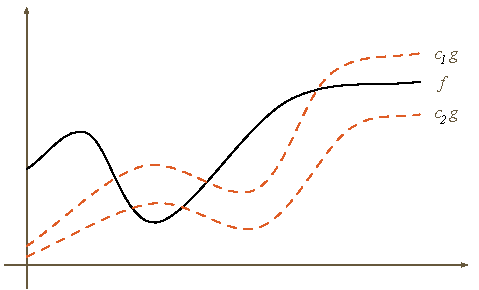
\includegraphics[scale=.5]{figures/asymptotic-theta.pdf}
    \end{figure}
%
  \end{itemize}
%
\end{frame}

% --------------------------------------
% upper and lower bounds
\begin{frame}[fragile]
%
  \frametitle{Upper and lower bounds}
%
  \begin{itemize}
%
  \item bounded from above: we say that $f = O(g)$ if there is a constant $c$ such that 
    $f(n) \leq c g(n)$ for sufficiently large $n$
%
    \begin{figure}
      \centering
      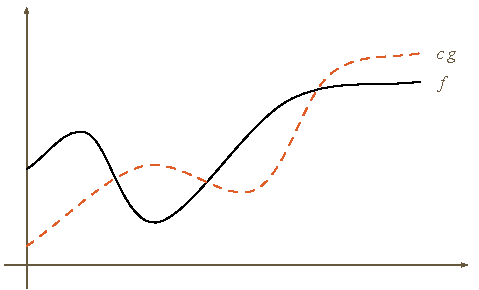
\includegraphics[scale=.5]{figures/asymptotic-o.pdf}
    \end{figure}
%
  \item bounded from below: we say that $f = \Omega(g)$ if there is a constant $c$ such that 
    $c g(n) \leq f(n)$ for sufficiently large $n$
%
    \begin{figure}
      \centering
      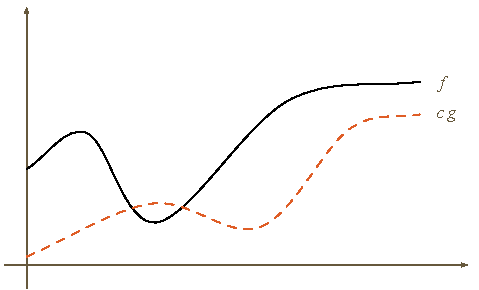
\includegraphics[scale=.5]{figures/asymptotic-omega.pdf}
    \end{figure}
%
  \end{itemize}
%
\end{frame}

% --------------------------------------
% algorithm design strategies
\begin{frame}[fragile]
%
  \frametitle{Designing algorithms}
%
  \begin{itemize}
%
  \item \insertionsort\ is {\em incremental}:
    \begin{itemize}
      \item having sorted $S[i..j]$, put $S[j]$ in its proper place
      \item how would you break this up into tasks that can be executed in parallel?
    \end{itemize}
%
  \item one alternative is {\em divide-and-conquer}: \mergesort
    \begin{itemize}
      \item {\em divide}: split $S$ into two parts of roughly equal length
      \item {\em conquer}: sort the subsequences recursively
      \item {\em combine}: merge the two sorted subsequences to produce the sorted output
    \end{itemize}
%
  \end{itemize}
%
\end{frame}

% --------------------------------------
% merge sort
\begin{frame}[fragile]
%
  \frametitle{Sorting by divide-and-conquer}
%
    \begin{center}
      \begin{minipage}{.75\linewidth}
        \begin{algorithm}[H]
          \label{alg:merge-sort}
%
          \dontprintsemicolon
          %\nocaptionofalgo
          \setalcaphskip{0ex}
%
          \caption{\mergesort($S$, $p$, $r$)}
          \vspace{.5em}
%
          \If{$p < r$}{
            $q \leftarrow \lfloor (p+r)/2 \rfloor$ \;
            \mergesort($S$, $p$, $q$) \;
            \mergesort($S$, $q+1$, $r$) \;
            \merge($S$, $p$, $q$, $r$) \;
          }
%
          \vspace{.5em}
%
        \end{algorithm}
      \end{minipage}
    \end{center}
%
  \begin{itemize}
%
  \item {\em exercise}: write \merge; can be done in $\Theta(r-p+1)$
%
  \item analysis of running time:
    \begin{itemize}
    \item involves solving a recurrence relation
    \item worst case:
      \[
      T(n) = \left\{
      \begin{array}{ll}
        \Theta(1)         & {\rm if\ } n = 1 \\
        2T(n/2)+\Theta(n) & {\rm if\ } n > 1
      \end{array} \right\}
      \rightarrow \Theta(n \log n)
      \]
    \end{itemize}
%
  \item is this a better candidate for parallel sorting?
%
  \end{itemize}
%
\end{frame}

% end of file 
